\section{Introduction}
% depth normal is natural ability, without groud truth
Human beings are professional in recovering the 3D geometry of observed natural scenes at very detailed level in real time, even from a single image. 
More impressively, we leaned to achieved this ability only through visual perception of consecutive changing of outside world and ego-motion. 
Practically, being able to do reconstruction through unlabeled videos can be widely applied to billions of online  applications like augmented reality, finding 3D placeholder for advertisement \etc.

Therefore, letting computer achieve dense 3D reconstruction ability is the central problem of computer vision. One group of approaches is geometric based method by using feature matching, \eg structure from motion (SFM) \cite{} \etc, or color matching, \eg DTAM \cite{}, \etc. 
Since our world exists in 3D space and the images projection follows camera geometry, as long as the matching from corresponding frames are correct, we can exactly solve the 3D structure. 
However, theoretically, those methods does not explain why human can also do reconstruction from a single image by observing videos. In addition, they can easily fail once the feature matching is wrong, \eg when SIFT\cite{} meets a wall with white color. 
In summary, geometric based methods do not have the ability to discover new reconstruction cues using videos, and ignore the information from monocular images.

Another way to do 3D reconstruction is learning based method, where the reconstruction cues can be incrementally discovered and applied by keeping feeding in unobserved videos. Currently, with the development of pixel-wise prediction via deep learning such as fully convolutional network (FCN) \cite{}, supervised learning of depth, \eg \cite{}, achieved impressive results over public datasets like KITTI \cite{}, NYUv2 \cite{} and SUN3D \cite{}. 
Nevertheless, collecting ground truth depth is almost impossible for most online videos, where the learned models are hard to generalize. 
Thus, learning depth with unlabeled videos attracts lots of attention in recent years.
Garg \etal \cite{godard2016unsupervised} try to use FCN to predict depth from a single image, by using photometric matching from stereo pairs, and back-propagate the matching error to the network. Later works \cite{zhou2017unsupervised,Vijayanarasimhan17} extends to using information from consecutive video frames by introducing camera ego-motion. 
Although those unsupervised learning based methods are able to do single image reconstruction, the results are still far from satisfactory. As shown at the left of \figref{fig:intro}, the depth results from \cite{zhou2017unsupervised} does not well represent the structure of scene, especially when observing with computed normals. 
This is mostly due to photometric matching is ambiguous, \ie a color in source frames can be matched to multiple similar colors in target frames. Although researchers usually use smoothness of depth \cite{zhou2017unsupervised} to reduce the ambiguity, it is often a weak constraint over neighbor pixels, yielding non-reasonable normal results.

Our work falls in the scope of learning based 3D reconstruction with videos following the work of \cite{zhou2017unsupervised}, but is a step further towards learning a regularized 3D geometry with particular awareness of normal representation. 
We are motivated by the fact that human beings are able to explicitly point out the normal direction of each pixel in an image. Actually, we are more sensitive to normal than depth, \eg we could precisely point out the normal direction of a pixel while could roughly know the exact depth. 
Thus, we embed the normals representation inside the network as regularization layers, and enforce the prediction consistency with depth, which we will describe in \secref{sec:approach}.
There are several advantages by using explicit normal representation. First, it gives explicit understanding of normal for learned models.  Second, it provides higher order interaction between depth, which is beyond neighboring pair. 
%Last but not the least, additional relationship, such as Manhattan world \cite{}, could be easily integrated with nor.
As shown at right of \figref{fig:intro}, with the help of normal representation, our recovered geometry is comparably better. We did extensive experiments over the publish KITTI and NYUv2 dataset for 3D reconstruction, and show our algorithm can achieve relative 20$\%$ improvement over the state-of-the-art method on depth estimation and 10$\%$ improvement on predicted normals. More importantly, we converge much faster. These demonstrate the efficiency and effectiveness of our approach.
% recent work stereo, (eccv 2016, cvpr 2017), motion (cvpr 2017)
% matching can be easy, keep local structure for regularize depth is important,  

% normal is the most important structure that can explicit represent, no work on this

% we focus on 1: regularize depth, 2: explicit represent normal, 3: enforce the consistency

\subsection{Framework}
\figref{fig:pipeline} illustrate an overview of our learning approach. For training, we apply supervision based on view synthesis following \cite{zhou2017unsupervised}. The depth network takes only the target view as input, and
outputs a per-pixel depth map $\ve{D}_t$, based on which a normal map $\ve{N}_t$ is generated by the depth-to-normal layer. Then, given the $\ve{D}_t$ and $\ve{N}_t$, a new set of depth maps $\{\ve{D}_t^i\}_{i=1}^{N}$ are estimated by the normal-to-depth layer using local orthogonal compatibility between depth and normals. 
All the depth maps, combined with poses predicted from the pose network, are then used to inverse warp the source views to reconstruct the target view, where errors are back propagate through both layers. Here the normal representation naturally serves as a regularization for depth, and . For training loss, additional to the usually used photometric reconstruction loss, we also use smoothness over normal, which induce higher order interaction between pixels. 

Finally, after the model is trained, given a new image,  we first infer per-pixel depth value and then compute the normal value, yielding consistent prediction between the two.
% problem normal can be locally estimated , while depth need global.  Another brach purely for normal


\begin{figure}
\centering
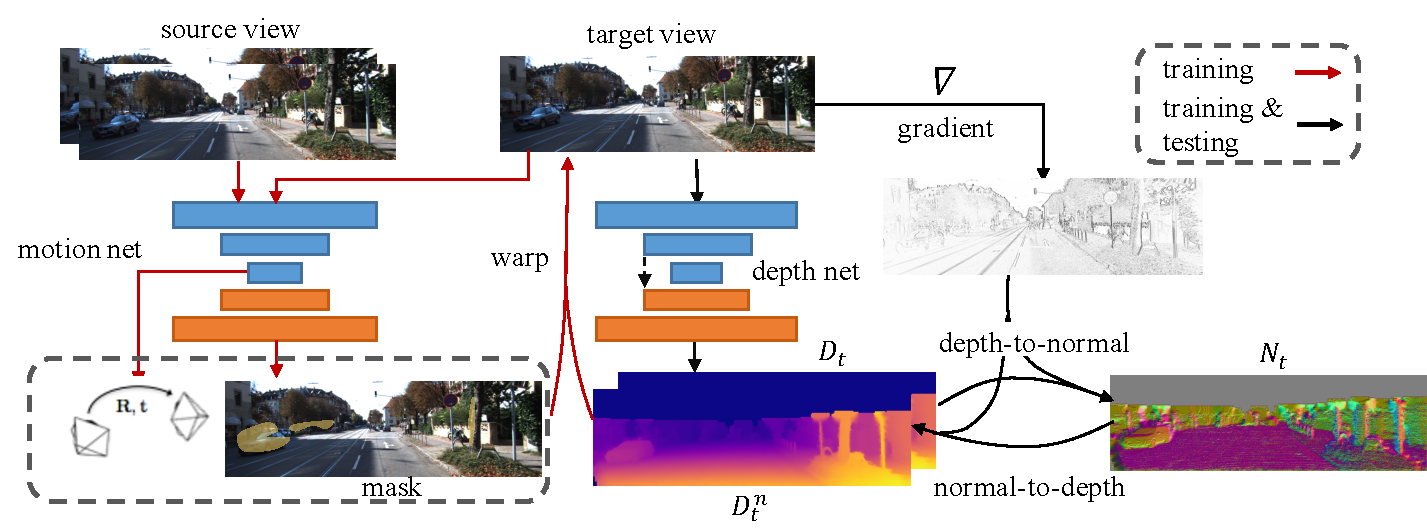
\includegraphics[width=\textwidth]{pipeline.png}
\caption{Framework.}
\label{fig:pipeline}
\end{figure}

% In summary, the contributions of this paper lie in three folds:
% \begin{enumerate}
%     \item We provide to explicitly represent normal from images via unsupervised depth estimation, which is useful in real applications and serves as a regularization for depth prediction.
%     \item We

% \end{enumerate}

